\item \points{15} {\bf Logistic Regression: Training stability}

In this problem, we will be delving deeper into the workings of logistic
regression. The goal of this problem is to help you develop your skills
debugging machine learning algorithms (which can be very different from
debugging software in general).

We have provided an implementation of logistic regression in
\texttt{src/stability/stability.py}, and two labeled datasets $A$ and $B$ in
\texttt{src/stability/ds1\_a.csv} and \texttt{src/stability/ds1\_b.csv}.

Please do not modify the code for the logistic regression training algorithm
for this problem. First, run the given logistic regression code to train two
different models on $A$ and $B$. You can run the code by simply executing
\texttt{python stability.py} in the \texttt{src/stability} directory.

\begin{enumerate}

  \item \subquestionpoints{2}
What is the most notable difference in training the logistic regression model
on datasets $A$ and $B$?


\ifnum\solutions=1 {
  \begin{answer}
	Our model converges on dataset A but fails to converge on dataset B. \\
\end{answer}

} \fi

  \item \subquestionpoints{5}
Investigate why the training procedure behaves unexpectedly on dataset $B$, but
not on $A$. Provide hard evidence (in the form of math, code, plots, etc.) to
corroborate your hypothesis for the misbehavior. Remember, you should address
why your explanation does \emph{not} apply to $A$.

\textbf{Hint}: The issue is not a numerical rounding or over/underflow error.


\ifnum\solutions=1 {
  \begin{answer}
	\begin{figure}[H]
	\centering
	\begin{subfigure}[H]{0.45\linewidth}
		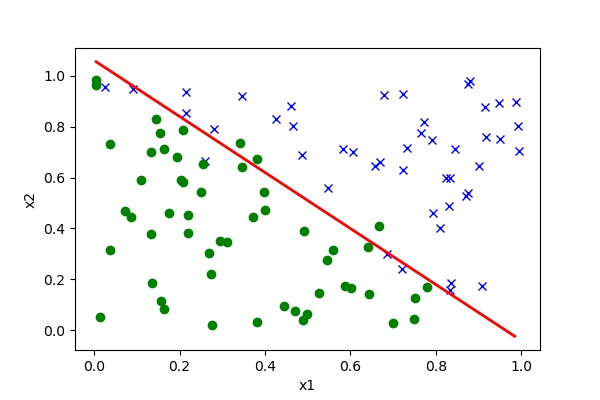
\includegraphics[width=\linewidth]{ds1_a}
		\caption{Dataset A isn't separable.}
	\end{subfigure}
	\begin{subfigure}[H]{0.45\linewidth}
		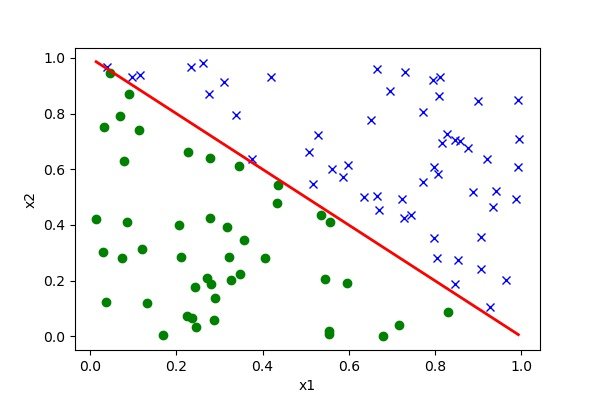
\includegraphics[width=\linewidth]{ds1_b}
		\caption{Dataset B separated by $ x_1 + x_2 = 1$.}
	\end{subfigure}
	\caption{These datasets differ in the linear separability.}
	\end{figure}
Let $\theta$ be a parameter vector such that dataset B is completely separated 
by the hyperplane $\theta^{T} x = 0$. Now, consider a parameter $\theta' = c 
\cdot \theta$. Given an example x, we observe that:
\begin{itemize}
	\item If $y=0$, then $\theta^{T} x < 0$ and its loss w.r.t. $\theta'$ is: 
	$-\log \left(\dfrac{1}{1 + \exp (-c\cdot\theta^T x)} \right)$.
	\item If $y=1$, then $\theta^T x > 0$ and its loss w.r.t. $\theta'$ is: 
	$-\log \left(1 - \dfrac{1}{1 + \exp (-c\cdot\theta^T x)} \right)$.
\end{itemize}
As $c \to \infty$, in both cases the losses are strictly decreasing without a 
bound. And so the total cost is a lower-unbounded convex function. The 
Gradient Descent will fail to converge to the global minimum since there is not 
such one. Due to inseparability, dataset A doesn't endure the above trait, our optimizer actually worked nicely. \\
\end{answer}

} \fi


  \item \subquestionpoints{5}
For each of these possible modifications, state whether or not it would lead to
the provided training algorithm converging on datasets such as $B$. Justify your
answers.
\begin{enumerate}
  \item Using a different constant learning rate.
  \item Decreasing the learning rate over time (e.g. scaling the initial
  learning rate by $1/t^2$, where $t$ is the number of gradient descent
  iterations thus far).
  \item Linear scaling of the input features.
  \item Adding a regularization term $\|\theta\|_2^2$ to the loss function.
  \item Adding zero-mean Gaussian noise to the training data or labels.
\end{enumerate}
 


\ifnum\solutions=1 {
  \begin{answer}
i., ii. Modifying the selection scheme for learning rates doesn't change the 
linear separability, hence the model wouldn't converge. \\
iii. Linear transformation doesn't remove the separability of dataset B, hence 
the model still wouldn't converge. \\
iv. Regularization can help in this case. The cost function is modified and 
might have a minimum now. \\
v. Adding noise terms might break the separability and make the model converge. 
\\
\end{answer}

} \fi


  \item \subquestionpoints{3} Are support vector machines vulnerable to datasets like $B$? Why or why not? Give an informal
justification.



\ifnum\solutions=1 {
  \begin{answer}
The Support Vector Machine is not vulnerable to separable datasets like B. The 
hard margin SVM actually dedicates to solve this problem. It tries to find 
a maximum margin classifier for such a dataset. \\
\end{answer}

} \fi

\end{enumerate}
